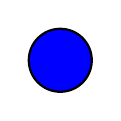
\begin{tikzpicture}

	% blue circle for hard scatter
	\def\hardScatterRadius{0.4}
	\draw[color = black, thick, fill = blue] (0, 0) circle (\hardScatterRadius);

	% small ellipse used for parton to hadron transistions
	\def\smallEllipseRx{0.1}
	\def\smallEllipseRy{3 * \smallEllipseRx}

	%\draw[color = black, thick, fill = green] (0, 1) circle [x radius = \smallEllipseRx, y radius = \smallEllipseRy];

\end{tikzpicture}
